\documentclass{article}

\usepackage{amsmath}
\usepackage{amssymb}
\usepackage{graphicx}
\usepackage{float}
\usepackage{mycommands}

 
\title{ECO220: Quantitative Methods in Economics \newline Lecture Notes (0201)}
\author{Tianyu Du, Instructor: Victor Yu}
\date{\today}

\begin{document}
	\maketitle
	\tableofcontents
	
	\section{Lecture 1 May. 08 2018}
	\subsection{Notations}
			\begin{center}
			\begin{tabular}{|c|c|c|}
				\hline
				Variable & Population & Sample \\
				\hline
				Size & $N$ & $n$ \\
				\hline
				Mean & $\mu$ & $\overline{x}$ \\
				\hline
				Std & $\sigma$ & $s$ \\
				\hline
			\end{tabular}
		\end{center}
	
	\subsection{From Sample to Population}
	\paragraph{} Let $p$ denote the percentage of qualified people in \underbar{population} and let $\hat{p}$ denote the percentage of qualified people in \underbar{sample}. Then, $p$ has an \underline{unknown} value and the value $\hat{p}$ can be calculated from sample data. We say \emph{$\hat{p}$ is an \textbf{estimator} for $p$}, and the value of $p$ is still unknown and can only be estimated.
	\paragraph{}$p$ is a \textbf{fixed value} (i.e. $p$ is fixed once population is fixed, we can measure the exact and certain value of $p$ if we traverse the whole population). But $\hat{p}$ will change from sample to sample. We call $\hat{p}$ an \textbf{estimator} (or \textbf{sample statistic}). The value of sample statistic will change from sample to sample. And, therefore, we call $\hat{p}$ a \textbf{random value}.
	
	
	\section{Lecture 2 May. 09 2018}
	\subsection{What is Statistics?}
		\[
			\text{Statistics}
				\begin{cases}
					\text{Descriptive Statistics}
						\begin{cases}
							\text{Graphs} \\
							\text{Numerical measures} \\
						\end{cases}
					\\
					\text{Inferential Statistics} \quad \emph{Draw conclusions in a population based on sample data.}
				\end{cases}
		\]
		\emph{Inferential Statistics involves uncertainties. To deal with the uncertainties, we need \textbf{probability}}
		\begin{figure*}[h]
			\centering
			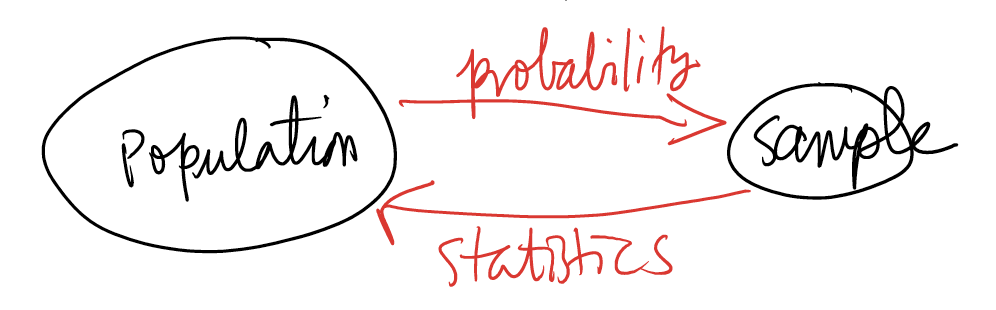
\includegraphics[width=0.6\linewidth]{fig1.png}
		\end{figure*}
		
	\subsection{Data}
		\[
			\text{Data}
			\begin{cases}
				\text{Quantitative data}
					\begin{cases}
						\text{Discrete}\\
						\text{Continuous}
					\end{cases}
					\\
				\text{Qualitative data (Categorical data)}
			\end{cases}
		\]
		
	\subsection{Descriptive Statistics - Graphs}
	
	\subsection{Descriptive Statistics - Numerical measures}
		\subsubsection{Measures of centre}
		\paragraph{Mean} Let $\sset{x}{1}{N}$ be measurements for the population with size $N$. The population mean is denoted by $\mu$ and defined as 
			\[
				\mu = \frac{1}{N}\sum_{i=1}^N{x_i}
			\]
		Let $\sset{x}{1}{n}$ be measurements for the \underbar{sample} of size $n$. The sample mean is denoted by $\overline{x}$ and defined as 
			\[
				\overline{x} = \frac{1}{n}\sum_{i=1}^n{x_i}
			\]
		\textbf{Note} \emph{The mean is sensitive to extreme values.}
		
		\paragraph{Median} is the value in the middle when all data are put in order of magnitude. (For data with even size, median is defined as the average of the two values in the middle.)
		
		\paragraph{Mode} is value(s) with highest frequency.
		
		\paragraph{Percentiles} the $k^{th}$ percentile is a number such that $k \%$ of data fall below this number.
		
		
	\section{Lecture 3 May. 15 2018}
		\subsection{Measures of Variation(Spread)}
		\paragraph{Variance and Standard Derivation} Let $\sset{x}{1}{N}$ denote the population with size $N$ and let $\sset{x}{1}{n}$ denote the sample with size $n$. Then
			\begin{center}
				\begin{tabular}{|c|c|c|}
					\hline
					Measures & Population & Sample \\
					\hline \hline
					Size & $N$ & $n$ \\
					\hline
					Mean & $\mu = \frac{1}{N}\sum_{i=1}^N{x_i}$ & $\overline{x} = \frac{1}{n}\sum_{i=1}^n{x_i}$ \\
					\hline
					Variance & $\sigma^2 = \frac{1}{N}\sum_{i=1}^N{(x_i - \mu)^2}$ & $s^2 = \frac{1}{n-1}\sum_{i=1}^n{(x_i-\overline{x})^2}$ \\
					\hline
					Std & $\sigma = + \sqrt{\sigma^2}$ & $s = +\sqrt{s^2}$ \\
					\hline 
				\end{tabular}
			\end{center}
			\paragraph{Note} When calculate the sample variance, use $n-1$ as denominator.
			\paragraph{Note} mathematically,
			\[
				s^2 = \frac{1}{n-1}\sum_{i=1}^n(x_i - \overline{x})^2 = \frac{1}{n-1}[\sum_{i=1}^n{x_i^2} - \frac{1}{n}(\sum_{i=1}^n{x_i})^2]
			\]
		\paragraph{Range} is defined as the difference between the largest value and the smallest value.
		
		\section{Lecture 4 May. 16 2018}
		\subsection{Covariance and Correlation: on Populations}
		\paragraph{} Consider two sets of data (population) with size $N$, denoted as $\sset{x}{1}{N}$ and $\sset{y}{1}{N}$, where $x$ and $y$ measure the age and income of observation, respectively.
		\paragraph{Denote} $\mu_x:=$ mean of $x$, $\mu_y:=$ mean of $y$\newline $\sigma_x:=$ std dev of $x$ and $\sigma_y:=$ std dev of $y$.
		\emph{When $x$ changes, does $y$ change?}
		\paragraph{Covariance} defined covariance between two datasets, $x$ and $y$ as,
			\[
				Cov(x,y) = \frac{1}{N}\sum_{i=1}^N{(x_i - \mu_x)(y_i - \mu_y)}
			\]
		\paragraph{Correlation coefficient} the correlation coefficient $\rho$ between datasets $x$ and $y$ is defined as
			\[
				\rho = \frac{Cov(x,y)}{\sigma_x \sigma_y}
			\]
			
		\subsection{Covariance and Correlation: on Samples}
		\paragraph{} When $N$ is too large, we select a sample of size $n$.
		\paragraph{} Let $\sset{x}{1}{n}$ and $\sset{y}{1}{n}$ denote the selected samples with size $n$, $\overline{x}, \overline{y}$ denote the sample means, and $s_x, s_y$ denote the sample std dev.
		\paragraph{Covariance} between two sample is defined as
			\[
				Cov(x,y) = \frac{1}{n-1}\sum_{i=1}^n{(x_i - \overline{x})(y_i - \overline{y})}
			\]
		\paragraph{Correlation coefficient} the sample correlation $r$ is defined as
			\[
				r = \frac{Cov(x,y)}{s_x s_y}
			\]
		\subsection{Interpretations}
		\subsubsection{Interpreting covariance}
			\paragraph{Example} Consider samples $x$ and $y$ with
				\[
					Cov(x,y) = -25.31
				\]
			The \underbar{negative sign} means $x$ and $y$ have a \underbar{negative linear relationship}. As $x$ increases, $y$ tends to decrease. The \underbar{magnitude} 25.31 has \textbf{no} meaning.
			
		\subsubsection{Interpreting correlation coefficient}
			\paragraph{Example} Consider samples $x$ and $y$ with
				\[
					r = -0.94
				\]
			The \underbar{negative sign} means $x$ and $y$ have \underbar{negative linear relationship}. As $x$ increases, $y$ decreases. The \underbar{magnitude} 0.94 means the \underbar{linear relationship is strong}. When $r$ is close to 1 or -1, the string line relation is strong, when $r$ is close to 0, the relation is weak.
			\paragraph{Note} $\rho \in [-1, 1]$ and $r \in [-1, 1]$
			
		\section{Lecture 5 May. 22 2018}
		\subsection{Introduction to Simple Regression}
		\paragraph{} Let the linear estimator to be $\hat{y} = b_0 + b_1 x$ and let $y_i$ denote the actual value at $x_i$, $\hat{y}$ is the estimated $y$ value at $x_i$. Then, $e_i := y_i - \hat{y_i}$ is the error of y value at $x_i$ (a.k.a. \textbf{residual}).
		\paragraph{Note} notice that $\sum_{i=1}^n{e_i} \equiv 0$.
		\paragraph{SSE} \textbf{Sum of Squared Error}(SSE) as
			\[
				SSE = \sum_{i=1}^n{e_i^2} = \sum_{i=1}^n(y_i - b_0 - b_1x_i)^2
			\]
		\paragraph{OLS} Minimize $SSE$ with respect to $b_0$ and $b_1$, we have the FOC as
			\[
				\begin{cases}
					\pd{SSE}{b_0} = 0 \\
					\pd{SSE}{b_1} = 0
				\end{cases}
			\]
			By solving the first order conditions, we have
			\[
				\begin{cases}
					b_1 = \frac{\sum(x_i - \overline{x})(y_i - \overline{y})}{\sum{(x_i - \overline{x})^2}} \\
					b_0 = \overline{y} - b_1 \overline{x}
				\end{cases}
			\]
			The above method to find $b_0$ and $b_1$ is called the \underbar{method of least square}, or \underbar{method of Ordinary Least Square (OLS)}.
			
		\subsection{Relationship between $b_1$ and $r$}
		\paragraph{}
			\[
				b_1 = \frac{Cov(x,y)}{Var(x)} = \frac{Cov(x,y)}{std(x)std(y)} \frac{std(y)}{std(x)} = r \frac{s_y}{s_x}
			\]
		
		\subsection{Analysis of Variance (ANOVA)}
		\paragraph{} Let $y_i$ denote the actual $y$ value at $x_i$ and $\hat{y_i}$ denote the estimated $y$ value at $x_i$.
		\paragraph{Definition}
			\[
				SST = \sum_{i=1}^n(y_i - \overline{y})^2
			\]
			\[
				SSR = \sum_{i=1}^n(\hat{y_i} - \overline{y})^2
			\]
			\[
				SSE = \sum_{i=1}^n(y_i - \hat{y_1})^2
			\]
		\paragraph{Notice} $SST = SSR + SSE$
		\paragraph{Anova Table}
		\begin{center}
			\begin{tabular} {|c|c|c|c|c|}
				\hline
				 & SS & df & MS & F \\
				 \hline
				 Regression & SSR & 1 & MSR & MSR/MSE \\
				 \hline
				 Error(Residual) & SSE & MSE & $n-2$ & \\
				 \hline
				 Total & SST & $n-1$ & & \\
				 \hline
			\end{tabular}
		\end{center}
		where MS stands for \textbf{mean square} and is defined as
			\[
				MS = \frac{SS}{df}
			\]
			\[
				MSR = \frac{SSR}{1}
			\]
			\[
				MSE = \frac{SSE}{n-2}
			\]
			
		\section{Lecture 6 May. 23 2018}
		\subsection{OLS, continued.}
		\paragraph{R-square} \textbf{coefficient of determination} is defined as 
			\[
				R^2 = \frac{SSR}{SST}
			\]
			and notice that $R^2 \in [0, 1]$ and can be interpreted as \textbf{\% of variation in $y$ explained by $x$ (via the linear model)}
		\paragraph{Note} in ECO220, we use $R^2$ or $r^2$ to represent the same thing.
		
		\subsection{Sample space, Event and Probability}
		\paragraph{Experiment} an experiment is a process that creates \underbar{two or more} outcomes.
		\paragraph{Random Experiment} a random experiment is an experiment such that the outputs \emph{cannot} be determined \underbar{with certainty} before the end of the experiment.
		\paragraph{Sample Space} a sample space is the \underbar{set} of all possible outcomes in a random experiment.
		\paragraph{Event} an event is a \underbar{subset} of a sample space.
		\paragraph{Prob} Let $S$ be the sample space, let $E$ be an event, then the \textbf{probability of $E$}, $P(E)$ is defined as
			\[
				P(E) = \tx{probability of $E$} = \frac{\tx{Number of outcomes in $E$}}{\tx{Number of outcomes in $S$}}
			\]
			\emph{assuming that each outcome in $S$ has \underbar{equal likelihood} to be chosen into $E$.}
			
		\subsection{Some Rules of Probability}
		\paragraph{} Let $E$ be an event in sample space $S$, then
		\begin{itemize}
			\item $P(E) \in [0, 1]$.
			\item $P(S) = 1$.
			\item Let $E^c$ denote the \textbf{complementary} of $E$, then $P(E^c) = 1 - P(E)$.
			\item $P(A \cup B) = P(A) + P(B) - P(A \cap B)$ (Addition Rule)
		\end{itemize}
		
	\section{Lecture 7 May. 29 2018}
		\paragraph{Mutually Exclusive Event} If $A\cap B = \emptyset$, we say events $A$ and $B$ are \textbf{mutually exclusive/disjoint}. Then, if $A,B$ are disjoint, we have 
			\[
				P(A\cup B) = P(A) + P(B)
			\]
			
		\subsection{Conditional Probability}
		\paragraph{Conditional Prob} In general, if $A$ and $B$ are events in sample space $S$, the \underbar{conditional probability of $A$ given $B$} is defined as 
			\[
				P(A \vert B) = \frac{P(A \cap B)}{P(B)}
			\]
		\paragraph{Multiplication rule}
			\[
				P(A \cap B) = P(A \vert B) P(B) = P(B \vert A) P(A)
			\]
		
		\subsection{Independent Event}
		\paragraph{Independent Event} We say two events, $A$ and $B$ are \textbf{independent} if any of the following is true. (those definitions below are equivalent.)
			\begin{itemize}
				\item $P(A \vert B) = P(A)$ or
				\item $P(B \vert A) = P(B)$ or
				\item $P(A \cap B) = P(A) P(B)$
			\end{itemize}
			
	\section{Lecture 8 May. 30 2018}
		\subsection{Bayes Theorem}
		\paragraph{} Let $A$ and $B$ be two events. Then,
		\[
			P(B\vert A) = \frac{P(A \vert B)P(B)}{P(A)}
		\]
		\emph{Proven by definition of conditional probability.}
		
		\subsection{Random Variable and Prob. Distributions}
		\paragraph{Prob. distribution}
		\paragraph{Cumulative Prob. distribution}
		
		\subsection{Expected Values}
		\paragraph{Expected Value} Let $X$ be a random variable with probability distribution $P(X)$. Then defined the expected value of $X$, $\mathbb{E}(X)$ as 
			\[
				\mu = \mathbb{E}(X) = \sum_{x}{x P(X=x)}
			\]
		\paragraph{Variance of Random Variable} For random variable $X$, we have
			\[
				\sigma^2 = Var(X) = \sum_{x}{(x - \mu)^2P(X=x)} = \mathbb{E}(X-\mu)^2
			\]
			
	\section{Lecture 9 June. 5 2018}
		\subsection{Expected Value of a Random Variable}
			\paragraph{Mean} $\mu = \mathbb{E}(X) = \sum_{x}{xP(X=x)}$.
			\paragraph{Variance} $\sigma^2 = \mathbb{E}(x - \mu)^2 = \mathbb{E}(X^2) - \mu^2$.
		\subsection{Laws of Expectation}
			\paragraph{} In general, let $X$ be a random variable, and let $a, c \in \R$, then
				\[
					\expect{aX+c} = a \expect{X} + c
				\]
				\[
					Var(aX+c) = Var(aX) = a^2 Var(X)
				\]
			\paragraph{} Let $X$ and $Y$ be random variables, and let $a,b,c \in \R$, then
				\[
					\expect{aX+bY+c} = a\expect{X} + b\expect{Y} + c
				\]
				\[
					Var(aX+bY+c) = Var(aX + bY) = a^2 Var(X) + b^2 Var(Y) + 2ab\ Cov(X,Y)
				\]
			\paragraph{Note} if $X$ and $Y$ are independent, then $\rho = Cov(X,Y) = 0$ and 
				\[
					Var(aX+bY+c) = a^2 Var(X) + b^2 Var(Y)
				\]
				
		\subsection{Binomial Distribution}
			\paragraph{} In general, let $n$ be the number of independent trails and $p = P(\#success)$. Let $X$ be a random variable which is the number of successes in $n$ trails, we have
			\[
				P(X=x) = \begin{pmatrix}
					n \\
					x
				\end{pmatrix} p^x (1-p)^{n-x},\tx{ for } x = \{0,1,2,\dots,n\}
			\]
			\[
				\mu = \expect{X} = np
			\]
			\[
				\sigma^2 = Var(X) = npq,\ q = 1-p
			\]
		
	\section{Lecture 10 June. 6 2018}
		\subsection{Uniform Distribution}
			\paragraph{} Let $X$ be uniform from $a$ to $b$. $f(x) = \frac{1}{b-a}, a \leq x \leq b$
			\[
				\mu = \expect{X} = \int_a^b{xf(x)dx} = \frac{a+b}{2}
			\]
			\[
				\sigma^2 = Var(X) = \expect{X^2} - \mu^2
			\]
		\subsection{Normal Distribution}
			\paragraph{} Let $X$ be a continuous random variable, satisfying $-\infty < x < \infty$. The mean of $X$ is $\mu$ and the variance of $X$ is $\sigma^2$. The graph of $X$ is
			\begin{figure*}[h]
				\centering
				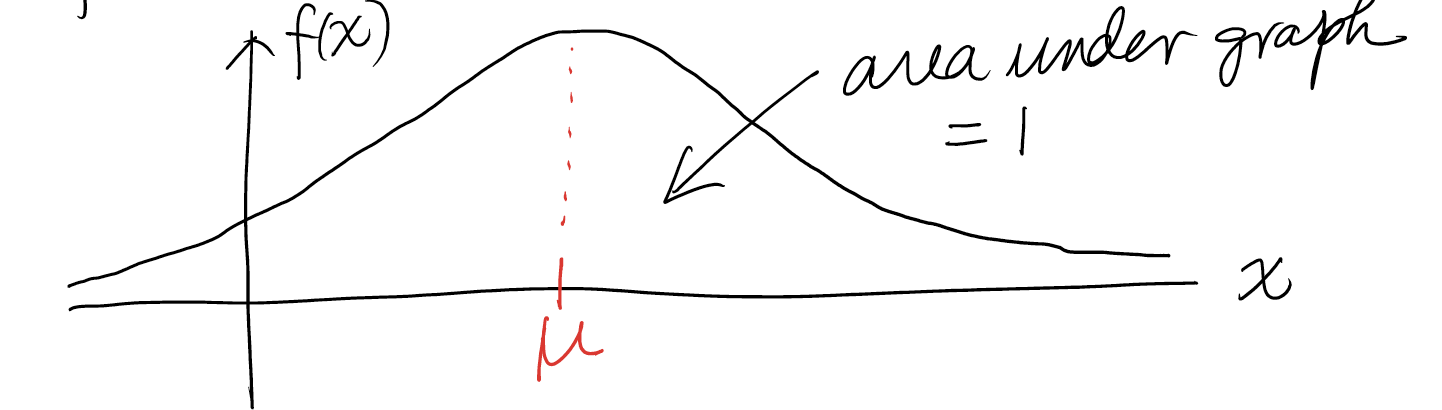
\includegraphics[width=0.6\linewidth]{fig2.png}
			\end{figure*}
			The graph is symmetric at $\mu$ and the variance $\sigma^2$ determines the shape(spread) of $X$. We say $X$ \underbar{follows a normal distribution with mean $\mu$ and variance $\sigma^2$.} And denote as 
				\[
					X \sim N(\mu, \sigma^2)
				\]
			\paragraph{Standard Normal Distribution} A standard normal distribution is a normal distribution with mean $\mu=0$ and standard deviation $\sigma=1$. Denote the standard normal distribution as
				\[
					Z \sim N(0,1)
				\]
	\section{Lecture 11 June. 12 2018}
		\subsection{Applying normal distribution}
			\paragraph{Theorem} Let $X \sim N(\mu, \sigma^2)$, then
				\[
					z = \frac{x - \mu}{\sigma} \sim N(0, 1)
				\]
		\subsection{Normal Approximation to Binomial}
			\paragraph{} Consider a random variable $X \sim B(n,p)$, then we can approximate the binomial with a normal distribution $X \approx N(np, npq)$.
	
	\section{Lecture 12 June. 13 2018}
		\subsection{Sampling Distributions}
			\paragraph{} Consider population with size $N$ has $p$ as percentage of \emph{success} (qualified) and sample with size $n$ with $\hat{p}=\frac{x}{n}$ as percentage of \emph{success}.
			\paragraph{} $p$ is a parameter which has a fixed value. In real life, the value of $p$ is usually unknown. $\hat{p}$ is a sample statistic, which does not have fixed value (random variable, value of $\hat{p}$ vary from sample to sample). Also, $\mu$ and $\sigma$ are parameters, which are fixed but usually unknown. $\overline{x}$ is a sample statistic, and is random.
			\paragraph{} Suppose we know $p$ for population, then we can conclude about random variables from a random sample,
				\begin{enumerate}
					\item $\expect{\hat{p}} = p$.
					\item $Var(\hat{p}) = \frac{pq}{n},\ q = 1-p$
					\item When sample size $n$ is large, the distribution of $\hat{p}$ is \underbar{approximately normal} (\textbf{Central Limit Theorem in proportion}) \footnote{As a rule of thumb, $n$ is considered to be large when $np\geq 10 \land nq \geq 10$.}
				\end{enumerate}
				That's
					\[
						\hat{p} \approx \sim N(p, \frac{pq}{n}),\ \tx{when $n$ is large.}
					\]
			\paragraph{Example} Given $p_{success} = 0.3$ for the whole population and find the probability that at least 320 \emph{success}  found in a sample of size $n=1000$. i.e. Let $X$ denote the number of success in sample with $n=1000$, find $P(X \geq 320)$.
			\paragraph{Method 1} Use Central Limit Theorem, check $np=300\geq10 \land nq = 700 \geq 10$, thus $n$ is \emph{large}. And approximate $\hat{p}$ of sample as
				\[
					\hat{p} \sim N(p, \frac{pq}{n})
				\]
				\begin{multline*}
					\emph{Soln.} \\
					P(X \geq 320) = P(\hat{p} \geq 0.32) \\
					= P(\frac{\hat{p} - p}{\sqrt{\frac{pq}{n}}} \geq \frac{0.32 - 0.3}{\sqrt{\frac{0.3*0.7}{1000}}}) = P(z \geq \frac{0.02}{\sqrt{\frac{0.21}{1000}}}) \\
					\tx{Find $z$ in z-table} \\
					\blacksquare
				\end{multline*}
			
			\paragraph{Method 2} Use Normal Approximation to Binomial. $p=0.3$ and $n=1000$.
			\[
				X \approx Y \sim N(300, 210)
			\]
			\begin{multline*}
				\emph{Soln.} \\
				P(X \geq 320) = P(Y > 319.5) \\
				= P(\frac{Y - \mu}{\sigma} > \frac{319.5 - 300}{\sqrt{210}}) \\
				= P(z > 1.35) \tx{ find in z table} \\
				\blacksquare
			\end{multline*}
			\paragraph{Note} \emph{methods 1 and 2 do \textbf{not} give exactly same answer, but the answers should be close.}
			
		\subsection{Sampling distribution of $\overline{X}$, the sample mean}
			\begin{enumerate}
				\item $\expect{\overline{X}} = \mu$.
				\item $Var(\overline{X}) = \frac{\sigma^2}{n}$.
				\item When $n$ is large, the distribution of $\overline{X}$ is approximately normal. (\textbf{Central Limit Theorem in Mean}).
				\item When population is normal, the distribution of $\overline{X}$ is exactly normal, regardless of the sample size $n$.
			\end{enumerate}
			Putting together,
				\[
					\overline{X} \sim N(\mu, \frac{\sigma^2}{n}), \tx{ when $n$ is large.}
				\]
				
	\section{Lecture 13 Jun. 19 2018}
		\subsection{Confidence Interval}
			\paragraph{} To find $100(1-\alpha)\%$ confidence interval for $p$ estimated from $\hat{p}$ is
			\[
				\hat{p} \pm z_{\frac{\alpha}{2}}\sqrt{\frac{\hat{p}\hat{q}}{n}}
			\]
		
		\subsection{Sample Size Required}
			\paragraph{} When we specify the confidence level $1-\alpha$, and the margin of error, the required sample size is
			\[
				n = \frac{z_{\frac{\alpha}{2}}^2}{(ME)^2}pq
			\]
			If $p$ can be estimated from previous surveys, use it to find $n$. Else, use $p=0.5$ to find $n$.
			
	\section{Lecture 14 Jul. 3 2018}
		\subsection{Confidence Interval for Population Proportion}
			\paragraph{} \textbf{Point estimator} for $p$ is $\hat{p}$, confidence interval for $p$ is 
				\[
					\hat{p} \pm z_{\alpha/2} \sqrt{\frac{\hat{p}\hat{q}}{n}},\ with\ large\ n
				\]
				$n$ is considered as \emph{large} iff $np \geq 10 \land nq \geq 10$.
				$\sqrt{\frac{\hat{p}\hat{q}}{n}}$ is the \textbf{standard error/deviation} of estimation. 
				And $z_{\alpha/2} \sqrt{\frac{\hat{p}\hat{q}}{n}}$ is the \textbf{margin of error}. 
		\subsection{Two populations}
			\paragraph{}$p_1, p_2$ denote the qualification percentages for population 1 and 2. And $\hat{p_1}, \hat{p_2}$ denote the qualification percentages in samples with sample sizes
				$n_1, n_2$ from population 1 and 2.
			\paragraph{Point estimator}To estimate $p_1$ to $p_2$, we estimate $p_1 - p_2$.
			The point estimator for $p_1 - p_2$ is $\hat{p_1} - \hat{p_2}$.
			\paragraph{Interval estimator}The interval estimation for $p_1 - p_2$ is 
				\[
					PointEstimator \pm z_{\alpha /2} \times Std(PointEstimator)
				\]
				\[
					\hat{p_1} - \hat{p_2} \pm z_{\alpha /2} \times Std(\hat{p_1} - \hat{p_2})
				\]
				To find $Std(\hat{p_1} - \hat{p_2})$, by \emph{law of expectation}
				\[
					Var(aX+bY) = Var(aX) + Var(bY) + 2abCov(X,Y)
				\]
				We select two independent samples of size $n_1$ and $n_2$ from populations, therefore
				\[
					V(\hat{p_1} - \hat{p_2}) = V(\hat{p_1}) + V(\hat{p_2})
				\]
				When $n_1$ and $n_2$ are \underline{large}, by \emph{central limit theorem}, 
				\begin{displaymath}
					\hat{p_1} \sim N(p_1, \frac{p_1 q_1}{n_1}), \quad
					\hat{p_2} \sim N(p_2, \frac{p_2 q_2}{n_2})
				\end{displaymath}
				Then, for two \emph{independent} samples, $\hat{p_1}$ and $\hat{p_2}$ are independent, 
				\[
					V(\hat{p_1} - \hat{p_2}) = \frac{p_1 q_1}{n_1} + \frac{p_2 q_2}{n_2}
				\]
				But we do not know $p_1$ and $p_2$, we cannot calculate $V(\hat{p_1} - \hat{p_2})$ directly from above equation. We estimate $p_1$ and $p_2$ by $\hat{p_1}$ and $\hat{p_2}$
				\newline Therefore the \textbf{estimated variance} is 
				\[
					(Estimated)V(\hat{p_1} - \hat{p_2}) = \frac{\hat{p_1} \hat{q_1}}{n_1} + \frac{\hat{p_2} \hat{q_2}}{n_2}
				\]
				\[
					(Estimated)Std(\hat{p_1} - \hat{p_2}) = \sqrt{\frac{\hat{p_1} \hat{q_1}}{n_1} + \frac{\hat{p_2} \hat{q_2}}{n_2}}
				\]
		\paragraph{Result} confidence interval for $\hat{p_1} - \hat{p_2}$
			\[
				C.I._{\alpha} = \hat{p_1} - \hat{p_2} \pm z_{\alpha/2} \sqrt{\frac{\hat{p_1} \hat{q_1}}{n_1} + \frac{\hat{p_2} \hat{q_2}}{n_2}}
			\]
		\paragraph{Example} Compare the percentage of people going to casino in Ontario and Manitoba.
			\begin{center}
				\begin{tabular}{l|cc}
				  Var & Ontario & Manitoba \\
				  \hline
				  Actual & $p_1$ & $p_2$ \\
				  Sample size & $n_1=4151$ & $n_2=389$ \\
				  Point estimator & $\hat{p_1}=66.5\%$ & $\hat{p_2}=75.2\%$
				\end{tabular}
			\end{center}
			\quad \textbf{Point estimator} for $p_1 - p_2$ is $\hat{p_1} - \hat{p_2} = -0.087$
			\newline the 95\% C.I. for $p_1 - p_2$ is
				\[
					-.0087 \pm (z_{.025}=1.96) * \sqrt{\frac{.665 * .335}{4151} + \frac{.752 * .248}{389}} = (-.132, -.042)
				\]
			\newline \textbf{Interpretation} 95\% of the times, $p_1 - p_2$ falls between -.132 and -.042. We are 95\% confident that $p_1 - p_2$ is between -.132 and -.042.
			\newline \textbf{Remark} Is there a \underbar{significant difference} between the \% going to casinos between Ontario and Manitoba? Since the 95\% C.I. for $p_1 - p_2$ does not contain 0, we conclude that there \textbf{is} a significant difference between \% in two population.
			\newline \textbf{Remark} You can also use estimate the $p_2 - p_1$ and the 95\% C.I. would be $(.042, .132)$.
		
		\subsection{Chapter 12. Hypothesis Testing in Population Proportion}
		\[
			\tx{Statistical Inference}
			\begin{cases}
				\tx{Estimation}
					\begin{cases}	
						\tx{Point Estimation} \\
						\tx{Interval Estimation}
					\end{cases}\\
				\tx{Hypothesis Testing}
			\end{cases}
		\]
		\paragraph{} $H_0$: the \textbf{null hypothesis}. $H_1$: the \textbf{alternative hypothesis}.
		\paragraph{Reality}
			\[
				\begin{cases}
					H_0 \tx{ Person not murder}
						\begin{cases}
							Guilty\ \vert \ H_0\textbf{ Type I Error}\\
							NotGuilty\ \vert \ H_0 \textbf{ No error}
						\end{cases} \\
					H_1 \tx{ Person is murderer}
						\begin{cases}
							Guilty\ \vert \ H_1 \textbf{ No error}\\
							NotGuilty\ \vert \ H_1 \textbf{ Type II Error}\\
						\end{cases}
				\end{cases}
			\]
		\paragraph{}When the court concludes "Guilty" and $H_0$ is true, type I error occurs and denote the probability of type I error as $\alpha$
			\[
				\alpha = P(\tx{Reject $H_0$} \vert H_0) P(\tx{Type I Error})
			\]
			And in this case, Type II Error will not occur.
		\paragraph{}Let $\beta$ denote the probability for type II error to occur.
			\[
				\beta = P(\tx{Reject $H_1$/Fail to reject $H_0$} \vert H_1) = P(\tx{Type II Error})
			\]
		\paragraph{Remark} $\beta$ becomes large as $\alpha$ becomes small. 
		\paragraph{Conclusion} Therefore, in \emph{hypothesis testing}, we have two hypotheses, $H_0$ and $H_1$. Based on sample results (evidence), we either \emph{reject $H_0$} or \emph{do not reject $H_0$}
		
	\section{Lecture 15 Jul. 4 2018}
		\subsection{Recall: Concepts of Hypothesis Testing}
			\paragraph{Concepts} $H_0$ \textbf{null hypothesis} and $H_1$ \textbf{alternative hypothesis}
			
			\paragraph{Case I} Rejecting $H_0$ while $H_0$ is true. \underbar{Failed to accept null hypothesis $H_0$}.
				\[
					\alpha = P(\tx{Reject }H_0\ \vert \ H_0 \tx{ True})= \textbf{Significance Level}
				\]
				\emph{In real life, we want the \textbf{significance level} to be as low as possible.} And note that significance level is probability for \underbar{type I error} to occur when $H_0$ is true.
				
			\paragraph{Case II} Accepting $H_0$ with $H_1$ is true. \underbar{Fail to accept alternative hypothesis}. $\beta$ is the probability of \underbar{type II error} while $H_1$ is true.
				\[
					\beta = P(\tx{Accept }H_0\ \vert \ H_1 \tx{ True})
				\]
			\paragraph{Remark} In hypothesis testing, we wish both $\alpha$ and $\beta$ to be small. However, by setting the rule of decision making and lowering $\alpha$, $\beta$ goes higher.
		\subsection{Hypothesis Testing}
			\textbf{Steps}
			\begin{enumerate}
				\item Set up null and alternative hypotheses $H_0$ and $H_1$.
				\item Setup a decision rule.
				\item Test statistic.
				\item Conclusion.
			\end{enumerate}
			
		\subsection{Hypothesis Testing in Population Proportion}
			\paragraph{Data} Population proportion $p$. Select sample with sample size $n$ and sample proportion $\hat{p}$.
			\paragraph{} $H_0$ null hypothesis on $p$ and $H_1$ as the alternative hypothesis.
			
			\paragraph{Example} Government claims that more than $50\%$ of Canadian are in favour of a policy.
			\newline
			\textbf{Step 1} setup hypotheses \underbar{$H_0:= p \leq 0.5$ and $H_1 := p > 0.5$}
			\newline
			\textbf{Step 2} setup a decision rule \underbar{If $\hat{p} < c$ we accept $H_0$. If $\hat{p} \geq c$ we reject $H_0$.}
			\newline Consider $c=0.55$. Then in a random sample of $n=200, \hat{p} = \%$ in favour from sample. Decision rule is
			\[
				\begin{cases}
					\tx{Accept $H_0: p \leq 0.5$ if $\hat{p} < 0.55$} \\
					\tx{Accept $H_1: p > 0.5$ if $\hat{p} \geq 0.55$}
				\end{cases}
			\]
			\newline \textbf{Step 3} test statistic. In a sample of $n=200, \hat{p}=0.58$.
			\newline \textbf{Step 4} Conclusion: Reject $H_0$.
			
			\subsubsection{Finding Critical Value c}
				\paragraph{} Finding $\alpha$
					\[
						\alpha = P(\tx{Type I Error}) = P(\hat{p}\geq 0.55 \vert p \leq 0.5)
					\]
					By \underbar{central limit theorem}, when $n$ is large,
					\[
						\hat{p} \sim N(np, \frac{pq}{n})
					\]
					Then normalized data, 
					\[
						\alpha = p(z \geq \frac{0.05 \sqrt{200}}{0.5}) = 0.0793 \approx 8\%
					\]
					Therefore, by setting the critical value $c=0.55$, the probability of type I error, $\alpha = 0.08$.
					\newline
					Finding $\beta$
					\[
						\beta = P(\hat{p} < 0.55 \vert p > 0.5)
					\]
				\begin{figure*}[h]
					\begin{center}
						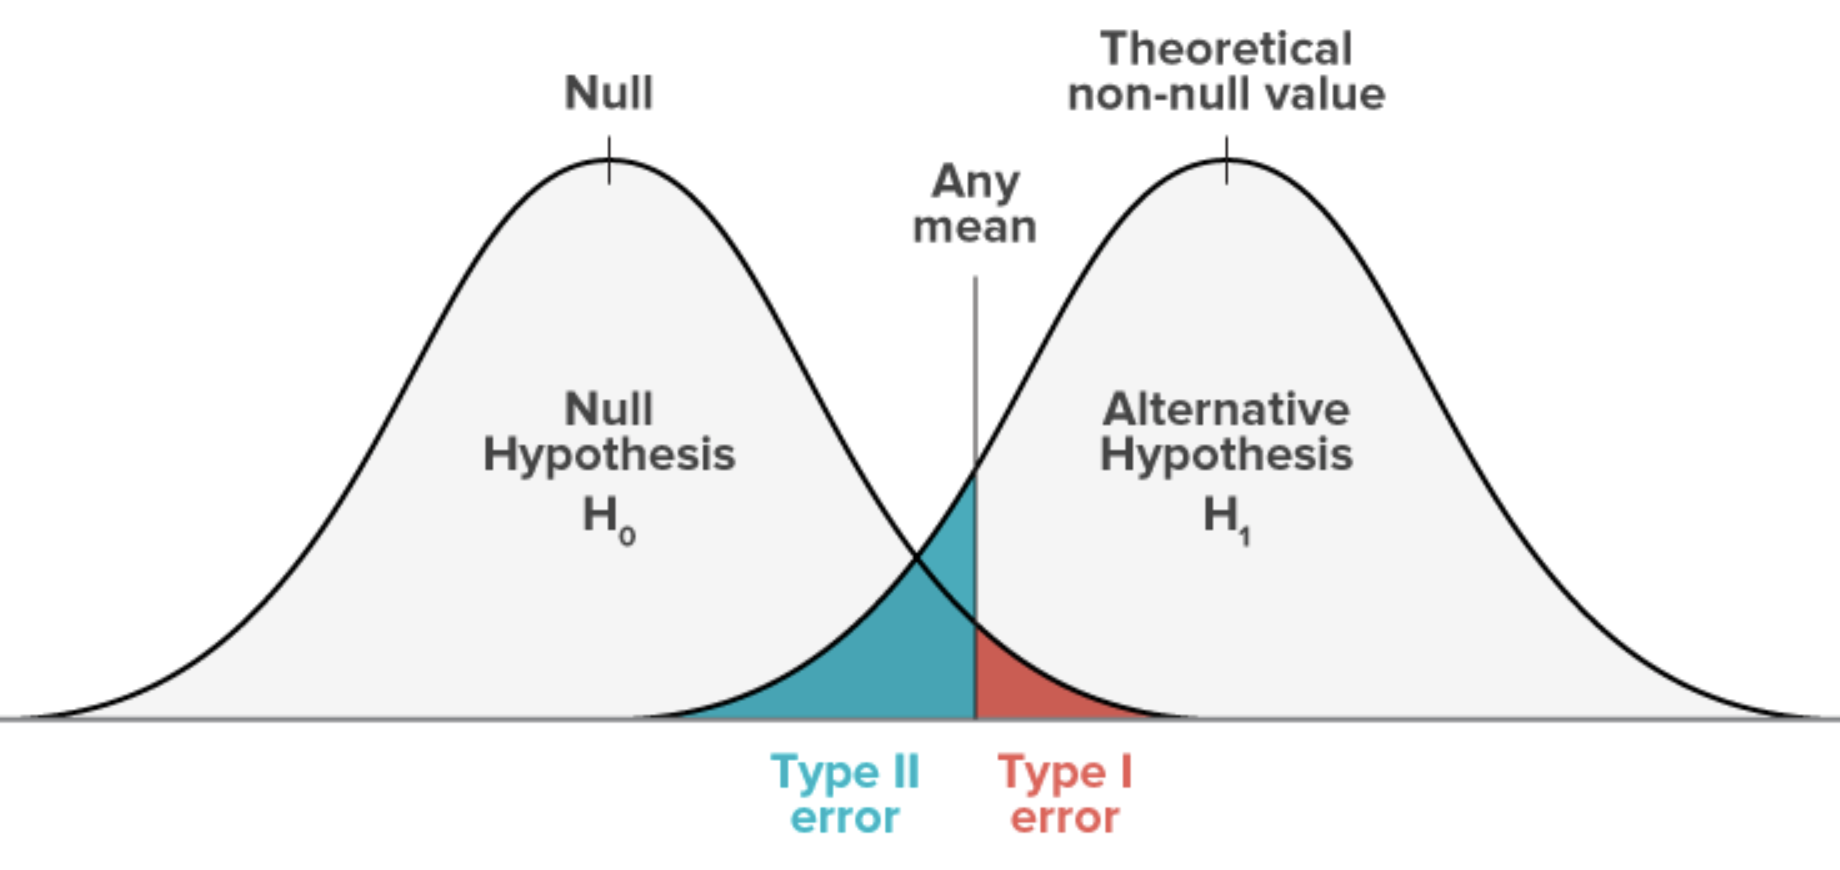
\includegraphics[width=\linewidth]{fig3}
					\end{center}
				\end{figure*}
\end{document}






















